\toptitle{[ELEC-H-201] Électricité et électronique}{TP2}
\TPtitle{Électricité et électronique\vspace*{2mm}}{TP2:\vspace*{2mm}
Réalisation d'un amplificateur audio - 1\up{ère} partie: analyse du montage}

\frontpage{consignes2.tex}
\vspace{5cm}
\newpage

\section{Manipulation}
\subsection{Définition du problème}
On désire réaliser un amplificateur dans la gamme des fréquences audio. Il sera utilisé pour amplifier le signal provenant de la sortie audio d'un ordinateur ou de votre téléphone\footnote{Étant donné que cette sortie est déjà amplifiée, afin qu'on puisse par
exemple y connecter une paire d'écouteurs, nous allons articiellement dégrader le signal
à l'aide d'un diviseur résistif.}, et piloter un haut-parleur (HP).\\

On dispose des informations suivantes (voir schéma en ANNEXE A):
\begin{itemize}
\item La plage des fréquences audio s'étend de $20Hz$ à $20kHz$.
\item Vous devez régler votre source pour qu'elle produise un signal d'environ 25 mV crête à la sortie du diviseur résistif, avec une impédance de sortie d'environ $100k\Omega$.
\item Le dernier étage ("étage de sortie") est un amplificateur de puissance ayant une sortie différentielle pour pouvoir connecter un haut-parleur.
\item Le haut-parleur (HP) se comporte comme une résistance de $16\Omega$ (impédance habituelle d'un HP)
dans la plage des fréquences audio. Sa puissance est limitée à $500mW$.
\item Le gain minimum de l'ampli audio doit idéalement valoir $0$ pour pouvoir annuler totalement le volume.
\end{itemize}

 \subsection{Découpage en blocs}

\Question{0}
{
%question
\textit{Dans le montage donné en ANNEXE A, identifiez les différents \textbf{composants} situés entre la source et l'amplificateur de puissance.}
}
{%assistant
Ampli-op, résistances, condensateurs, potentiomètres
}

Pour analyser un circuit électronique complexe, il est plus facile de commencer par identifier les différentes fonctions principales (amplification, filtrage, etc) réalisées dans ce circuit et de découper le montage en blocs. Ensuite, on pourra étudier ces différents blocs séparément. Selon la complexité du circuit, ces opérations pourront être itératives, c'est-à-dire qu'on pourra découper ces blocs en sous-blocs, etc.

\Question{0}
{
%question
\textit{Sur le schéma, identifiez et encadrez les différentes \textbf{fonctions} du montage.}
}
{%assistant
\begin{center}
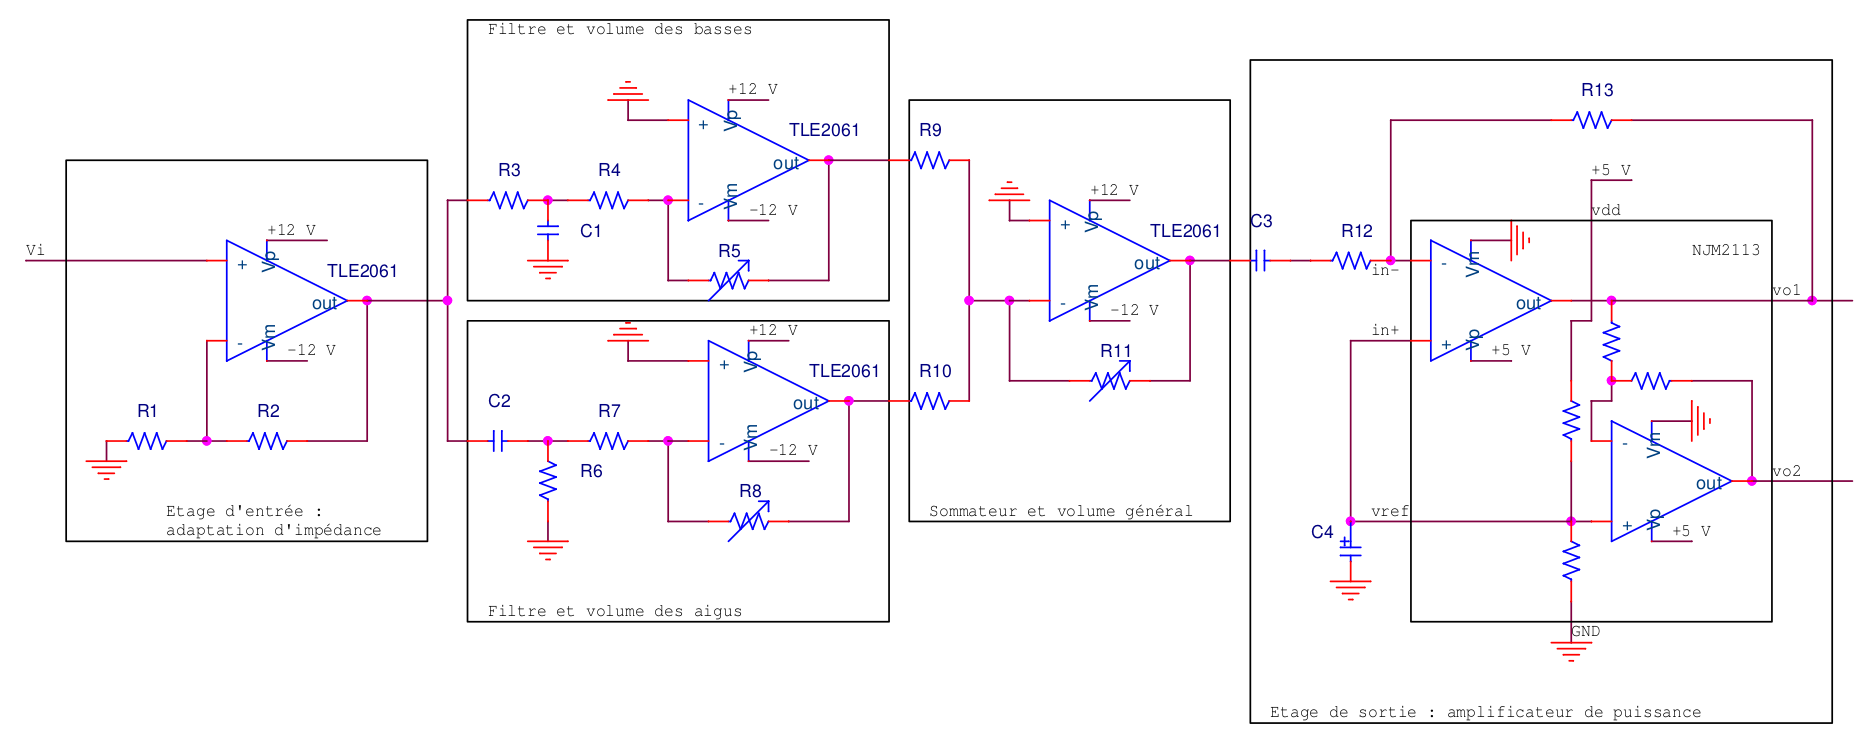
\includegraphics[width=\textwidth]{decoupageenblocs.PNG}
\label{decoupageenblocs}
\end{center}
}

\Question{0}
{
%question
\textit{Redessinez un schéma bloc du montage en y indiquant la fonctionnalité de chaque bloc.}
}
{%assistant
\begin{center}
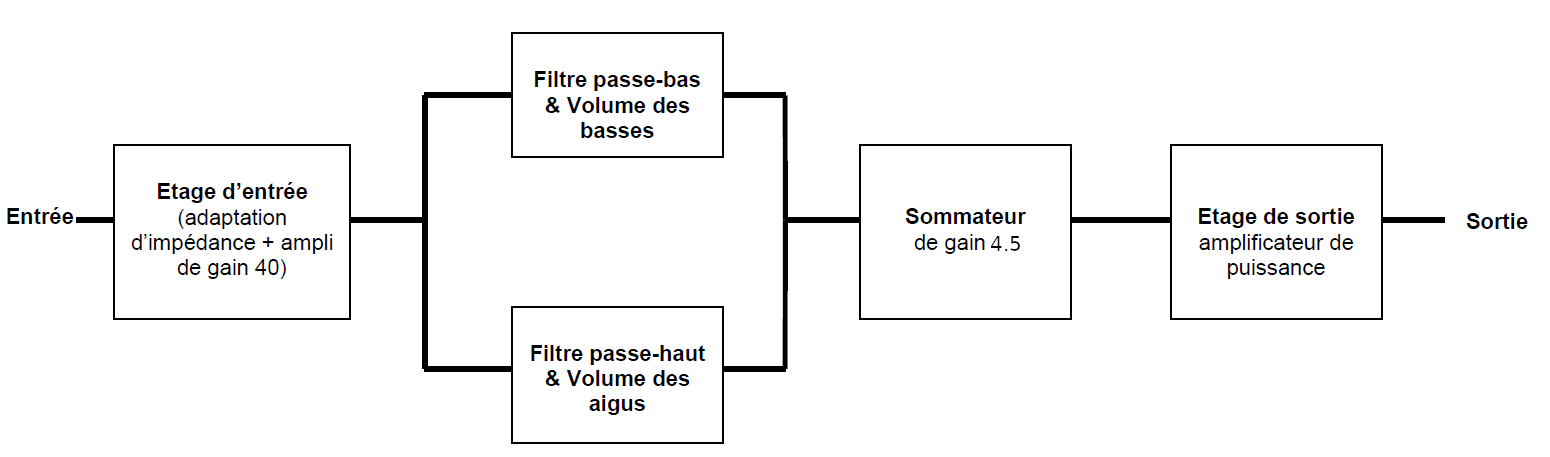
\includegraphics[scale=0.35]{fonctionsblocs.PNG}
\label{fonctionsblocs}
\end{center}
}

\subsection{Analyse préliminaire}
\label{analysepréliminaire}
Une propriété importante des ampli-op est leur produit "gain.bande passante". Le produit "gain.bande passante" d'un montage amplificateur à ampli-op est \textbf{constant}: si l'on augmente le gain du montage, la bande passante diminue et inversement (ceci est lié aux propriétés de la rétroaction - sans démonstration). Comme on va le voir, le produit "gain.bande passante" intervient dans le dimensionnement d'un montage à ampli-op.\\

Rappel: la bande passante est la plage de fréquence dans laquelle un circuit fonctionne sans que sa
sortie ne soit atténuée de plus d'un facteur $\sqrt{2}$.\\

Pour notre montage, nous avons choisi d'utiliser des ampli-op TLE2061.

\Question{0}
{
%question
\textit{A l’aide de la notice du constructeur (voir Annexe B), donnez le produit « gain bande passante », les impédances d'entrée et de sortie et le courant maximum de sortie de cet ampli-op.}
}
{%assistant
\begin{itemize}
\item $G.BW = 1,5MHz$
\item $Z_{in} = 10 T\Omega+4pF$
\item $Z_{out}=280\Omega$
\item $I_{{out}_{sortant}}=80mA$
\end{itemize}
}

\Question{0}
{
%question
\textit{Calculez le gain maximum d'un étage à TLE2061 qui respecte la bande passante voulue.}
}
{%assistant
$BW = 20kHz \Rightarrow G_{max} = 75$
}

\Question{0}
{
%question
\textit{A partir de cette dernière valeur, on peut déterminer le nombre minimum d'étages d'amplification.
\begin{itemize}
\item Pour cela, nous avons besoin de la valeur de crête maximum supportée par le HP. Déterminez-la.
\item Déduisez-en le gain maximum du montage.
\item A partir de ce gain maximum du montage et du gain maximum d'un étage, déterminez le nombre d'étages nécessaire.
\end{itemize}}
}
{%assistant
\begin{itemize}
\item $p=\frac{V_{eff}^2}{R} \Rightarrow V_{crete}^2=P\times R\times 2=16 \Rightarrow V_{crete}=4V$
\item $G_{max}=\frac{4V}{25mV}=160$
\item 2 étages nécessaires car $75^2=5625>160$
\end{itemize}
}

\subsection{1\up{er} étage}

\Question{0}
{
%question
\textit{Sur base du schéma, indiquez:
\begin{itemize}
\item Quel est le type de montage à ampli-op ?
\item Quel est le gain de cet étage ?
\item Sur base des caractéristiques de ce type de montage et de la source placée à son entrée, justifiez son choix.
\end{itemize}}
}
{%assistant
\begin{itemize}
\item Montage en non-inverseur
\item $G=1+\frac{R_2}{R_1} \Rightarrow G=40$
\item La résistance de sortie de la source est $100k\Omega$. Or pour avoir une adaptation d'impédance, on doit avoir $R_{source} << R_{in} \Rightarrow$ Montage non-inverseur.
\end{itemize}
}

\subsection{2\up{ème} étage}

\Question{0}
{
%question
\textit{Du point de vue adaptation d'impédance, est-il raisonnable de connecter ce second étage au premier ?}
}
{%assistant
Oui, tant que l'impédance d'entrée des montages en aval est beaucoup plus grande que $280\Omega$.
}

Le deuxième étage peut être divisé en deux blocs mis en parallèle qui eux-mêmes peuvent être divisés en deux sous-blocs. Le premier sous-bloc est un filtre et le second un ampli.
\Question{0}
{
%question
\textit{Quel est le type de montage à ampli-op ?}
}
{%assistant
Montage en inverseur
}

\Question{0}
{
%question
\textit{Respectons-nous bien l'adaptation d'impédance entre le filtre et l'ampli ?}
}
{%assistant
$R_{out} << R_{in}$
}

\Question{0}
{
%question
\textit{Quel est le gain de cet ampli ?}
}
{%assistant
$G_{max} = -1$
}

\Question{0}
{
%question
\textit{Pour quelle raison avons-nous choisi ce type de montage alors que l'autre type de montage aurait permis d'utiliser des résistances de plus faible valeur ?}
}
{%assistant
Pour pouvoir annuler les basses ou les aigus.
}

\Question{0}
{
%question
\textit{Quelle est la fréquence de coupure du filtre ?}
}
{%assistant
Pour calculer la fréquence de coupure du filtre, il faut tenir compte de l'impédance
d'entrée de l'ampli :
\begin{center}
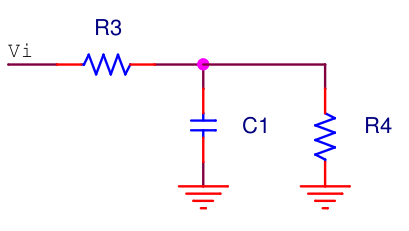
\includegraphics[scale=0.35]{filtre.PNG}
\label{fonctionsblocs}
\begin{tabular}{|c||c||c|}\hline
$R_3 = 2.7 k\Omega$ & $R_4 = 100 k\Omega$ & $C_1 = 100 nF$ \\ \hline
\end{tabular}
\end{center}
$$\omega = \frac{1}{\tau}\ et\ \omega=2\pi f \Rightarrow f=\frac{1}{2\pi \tau}\ avec\ \tau = RC$$
$$R=\frac{R_3 R_4}{R_3 + R_4}=2629\Omega \Rightarrow \tau = 2,63 \times 10^{-4}$$
$$\Rightarrow f = 605,15Hz$$

Autre méthode si on ne se souvient pas de la constante de temps:\\
La fréquence de coupure se produit, dans un circuit RC, quand l'impédance de la
résistance est égale (en norme) à l'impédance du condensateur :
$$|Z_R|=|Z_C|\Rightarrow R=\frac{1}{\omega C} \Rightarrow \omega =\frac{1}{RC} \Rightarrow f=\frac{1}{2\pi RC}$$
Il suffit donc de calculer $R$ comme précédemment pour trouver la réponse.
}

Pour quelle raison avons-nous choisi une telle fréquence de coupure? La première idée qui vient à l'esprit est de placer la fréquence de coupure au milieu de la bande audio ($20Hz$ à $20kHz$), pour la diviser en deux parts égales. La fréquence de coupure divisant basses et aigües serait alors de $10kHz$ environ.\\
C'est une bonne idée, mais il y a une subtilité : l'oreille humaine possède une sensibilité logarithmique à la fréquence: l'écart perçu par une oreille humaine entre deux notes ne dépend pas de la différence des deux fréquences mais du rapport de ces deux fréquences.\\
Pour s'en persuader, il suffit de regarder les fréquences des notes de musique. Elles sont organisées en octaves; une octave comprend 12 tons, également espacés; ils correspondent aux 12 touches d'un piano :
\begin{center}
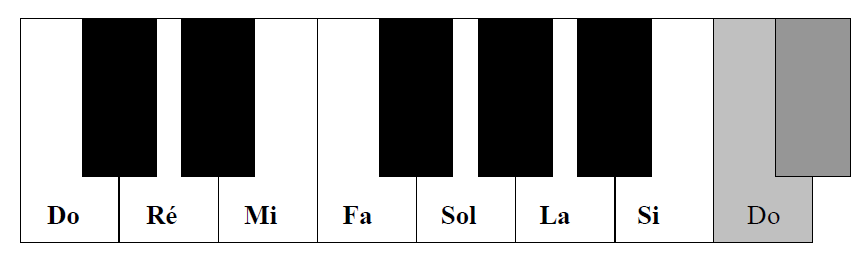
\includegraphics[scale=0.4]{piano.PNG}
\label{piano}
\end{center}

Le tableau ci-dessous donne les fréquences des notes de musique (en $Hz$), pour 2 octaves consécutives :
\begin{center}
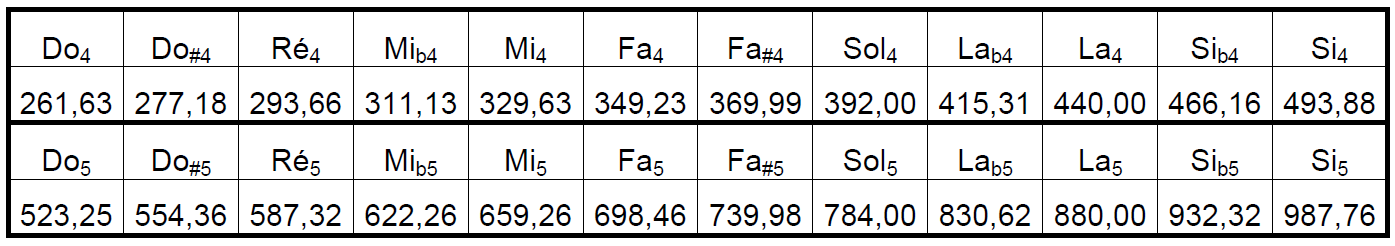
\includegraphics[scale=0.4]{notes.PNG}
\label{notes}
\end{center}

On voit que:
\begin{itemize}
\item d'une octave à l'autre, la fréquence a été multipliée par 2
\item d'un ton au suivant, la fréquence a été multipliée par $\sqrt[12]{2}$. La fréquence des notes de musique forme donc une suite géométrique de $\sqrt[12]{2}$.
\end{itemize}

De ceci, on peut déduire que la fréquence séparant les basses des aigus doit être la moyenne \emph{géométrique}\footnote{Rappel : moyenne géométrique de $a$ et de $b = \sqrt{a\times b}$} (et non la moyenne arithmétique) des fréquences extrêmes de la gamme audio. Les bonnes oreilles humaines entendent les notes depuis le $Do_0$ ($16,35Hz$) jusqu'au $Do_{10}$ ($16742Hz$), soit 10 octaves.\\
Une fréquence logique pour diviser cette gamme "en deux" (basses/aigües) est donc le $Do_5$.\\

N.B.: Une autre valeur "moyenne" possible est le $La_4$ ($440Hz$), la note sur laquelle on accorde les instruments; c'est aussi celle que vous entendez lorsque vous décrochez votre téléphone.

 \ifthenelse{\boolean{corrige}}{\newpage}{}
\subsection{3\up{ème} étage}

\Question{0}
{
%question
\textit{En considérant des tensions $V_{{i}_1}$ et $V_{{i}_2}$ entrant respectivement dans cet étage par les résistances $R_9$ et $R_{10}$, donnez la tension de sortie en fonction de $V_{{i}_1}$, $V_{{i}_2}$, $R_9$, $R_{10}$ et $R_{11}$. (indication : utiliser les théorèmes du zéro virtuel et de superposition)}
}
{%assistant
Nous allons utiliser le théorème de superposition. Commençons en ne considérant que
la source $V_{{i}_1}$ et remplaçons les sources de tension par des courts-circuits et les sources de courant par des circuits-ouverts.\\

En appliquant le théorème du zéro virtuel, l'entrée inverseuse de l’ampli-op est à $0V$. Ce qui implique qu'aucun courant ne circule dans la résistance $R_{10}$ puisque la différence de potentiel aux bornes de cette résistance est nulle.\\
Comme le courant ne peut rentrer par la borne inverseuse de l’ampli-op, on a $i_1 = i_2$, avec $i_1$ le courant circulant dans $R_9$ et $i_2$ celui dans
$R_{11}$, tous deux dirigés vers la droite du montage.
$$V_{o_1}=-i_2\times R_{11}\ et\ i_1=\frac{V_{{i}_1}}{R_9} \Rightarrow V_o=-\frac{R_{11}}{R_9}\times V_{{i}_1}$$
On peut refaire le même raisonnement pour la source $V_{{i}_2}$ et en remplaçant $V_{{i}_1}$ par un court-circuit. Ce qui donne:
$$V_{o_2}=-\frac{R_{11}}{R_{10}}\times V_{{i}_2}$$
Par le théorème de superposition, on obtient :
$$V_o=V_{o_1}+V_{o_2}=-\frac{R_{11}}{R_9}\times V_{{i}_1}-\frac{R_{11}}{R_{10}}\times V_{{i}_2}$$
Ce qui peut être simplifié du fait que $R_{10} = R_9$:
$$V_o=-\frac{R_{11}}{R_9}\times (V_{{i}_1}+V_{{i}_2})$$
}

\Question{0}
{
%question
\textit{Quel est la plage de gain ?}
}
{%assistant
De $0$ à $-20$ ($-\frac{R_{11}}{R_9}\cong -4.5$)
}

\subsection{Etage de sortie}
Les HP ne supportent pas qu'on leur applique des tensions continues; en effet, la partie électrique d'un HP est essentiellement composée d'une bobine dont l'impédance est quasi nulle en continu. Il faudra donc éliminer cette composante continue.
\subsubsection{Explication de l'amplificateur de puissance}
On peut remarquer que la résistance de charge est de faible valeur; cela implique qu'il faut pouvoir lui fournir un courant important :
$$I_{{out}_{max}}=\frac{V_{{out}_{max}}}{R_{HP}}=\frac{4V}{16\Omega}=250mA$$
Où $V_{{out}_{max}}$ est la valeur crête maximum supportée par le haut-parleur
calculée en \ref{analysepréliminaire}).\\

C'est beaucoup plus que ce que peut fournir un TLE2061. Il faut donc ajouter un 3\up{e} étage, appelé étage de sortie, dont le rôle est de fournir le courant nécessaire à la charge. Il existe des amplis-op spécialement conçus pour réaliser ces étages de sortie.\\
Les fabricants conseillent d'utiliser ces amplis-op dans des montages dont le gain est faible (typiquement A = 1), pour optimiser leurs performances. Leur but n'est donc pas d'amplifier une tension d'entrée, mais de fournir le courant nécessaire à la charge.\\

On utilisera l'ampli-op NJM2113; il peut fournir une puissance de $550mW$ à une charge de $16\Omega$. Il a été spécialement conçu pour les applications demandant une faible puissance sonore : GSM, baladeur, lecteur mp3, carte son,...\\
Malheureusement, ces appareils ne disposent en général que d'une source de tension de $5V$ (produite en régulant la tension de la batterie ou des piles); il est donc impossible d'alimenter les ampli-op de manière symétrique ($+12V/-12V$, $+5V/-5V$, etc). Le NJM2113 a donc été spécialement conçu pour être alimenté en
$+5V/0V$.\\
Cela a une conséquence importante (et gênante) : les limites d'écrêtage de l'ampli ne sont plus symétriques et en particulier, le signal de sortie ne peut plus devenir négatif.\\
On ne peut donc pas amplifier directement notre signal (qui est purement alternatif) avec cet ampli. On doit ajouter au signal une composante continue, pour que celui-ci ne devienne jamais négatif :
\begin{center}
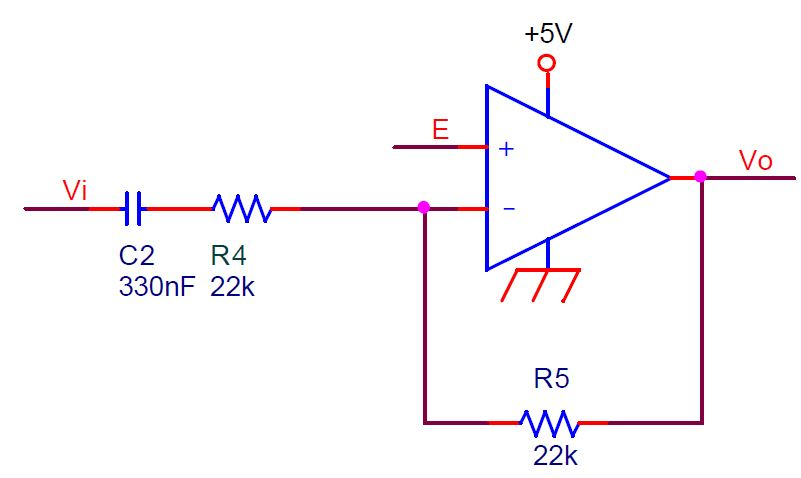
\includegraphics[scale=0.4]{polarisation.JPG}
\label{polarisation}
\end{center}

Dans le schéma ci-dessus, $V_i$ est le signal que l'on veut amplifier (signal utile) et $E$ est une tension continue (à déterminer) qui va empêcher la tension de sortie de devenir négative.\\
On a ajouté un condensateur en série avec l'entrée, pour supprimer l'éventuelle composante continue de $V_i$. Cet étage a donc un comportement de filtre passe-haut; sa fréquence de coupure est de $20Hz$.\\
Classiquement, on choisit la valeur de $E$ qui maximise l'amplitude admissible de $V_i$. Si $V_i$ est symétrique comme ici, $E$ doit être au milieu de la gamme d'alimentation de l'ampli-op ($0-5V$), donc $E = 2,5V$ pour permettre une valeur crête maximale de $V_i$ de $2,5V$ également.

\Question{0}
{
%question
\textit{En considérant la fréquence de $V_i$ supérieur à $20Hz$ telle que l'on puisse considérer le condensateur $C_2$ comme un court-circuit, montrez (par exemple en utilisant le principe de superposition) qu'on obtient $V_o = E - V_i$}
}
{%assistant
En utilisant de principe de superposition, on va travailler source par source, calculer la tension de sortie pour chaque cas et additionner les valeurs obtenues :
\begin{enumerate}
\item On va d'abord considérer uniquement la source $V_i$ (on annule donc $E$) : le montage se résume donc à un inverseur et $V_{o_1} = -\frac{R_5}{R_4}V_i = -Vi$
\item On va ensuite considérer uniquement la source continue $E$ (on annule donc $V_i$) : il faut faire attention au fait qu'en annulant $V_i$, la capacité $C_2$ joue le rôle d'un circuit ouvert et qu'aucun courant ne circule dans les résistances. De ce fait, le montage se résume à un suiveur pour la tension continue donc $V_{o_2} = E$
\item On additionne les tensions de sorties obtenues séparément :
$$V_o = V_{o_1} + V_{o_2} = E - V_i$$
\end{enumerate}
}

Avec ce montage, on arrive donc à amplifier notre signal d'entrée sans être gêné par les limites d'écrêtage de l'ampli-op. Ce montage a cependant un gros inconvénient : sa tension de sortie a une composante continue importante ($2,5V$); on ne peut donc connecter directement un HP à sa sortie.\\
On pourrait placer un condensateur entre la sortie de l'ampli et le HP pour créer un filtre passe-haut, mais la valeur de ce condensateur devrait être très élevée pour avoir une fréquence de coupure de $20Hz$ :
$$C=\frac{1}{2 \pi R_{HP} f_c}=995\mu F$$
$1mF$ est une valeur de capacité qui n'est pas irréaliste, mais qui est à la limite de ce qui est réalisable. Un condensateur de $1mF$ se présente typiquement sous la forme d'un cylindre de $1$ à $2cm$ de diamètre et de $4cm$ de hauteur; il s'agit donc d'un élément volumineux, peu adapté pour être inclus dans un appareil portable.
\newpage

Les concepteurs du NJM2113 ont donc imaginé une astuce pour éviter de devoir utiliser un tel condensateur :
\begin{center}
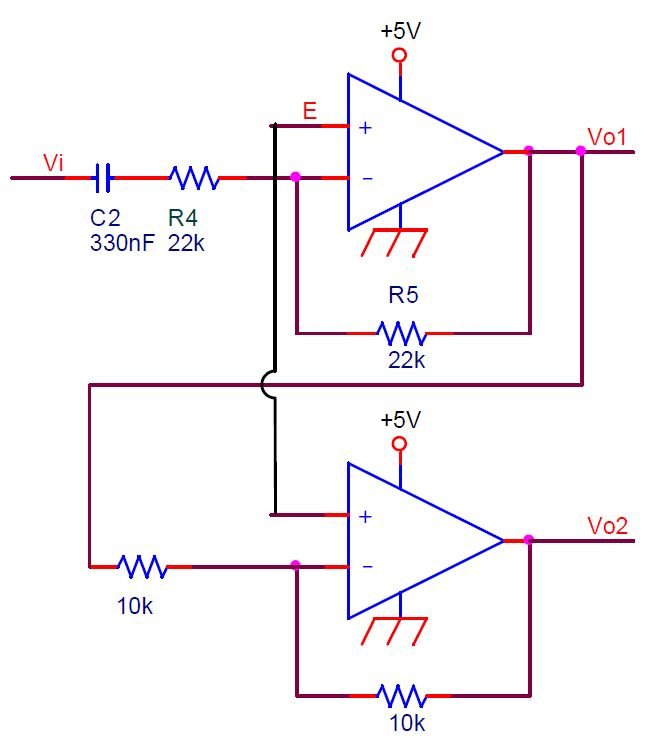
\includegraphics[scale=0.5]{astuceLM4864.JPG}
\label{astuceLM4864}
\end{center}
 On peut vérifier que:
 $$V_{o_1}=E-V_i\ et\ V_{o_2}=E+V_i \Rightarrow V_o=V_{o_2}-V_{o_1}=2V_i$$

En plaçant notre HP entre les sorties des deux amplis, on lui applique une tension purement alternative : puisque les deux tensions de sortie ont la même composante continue, ces dernières s'annulent.\\

Le circuit NJM2113 intègre presque toute cette solution :
\begin{center}
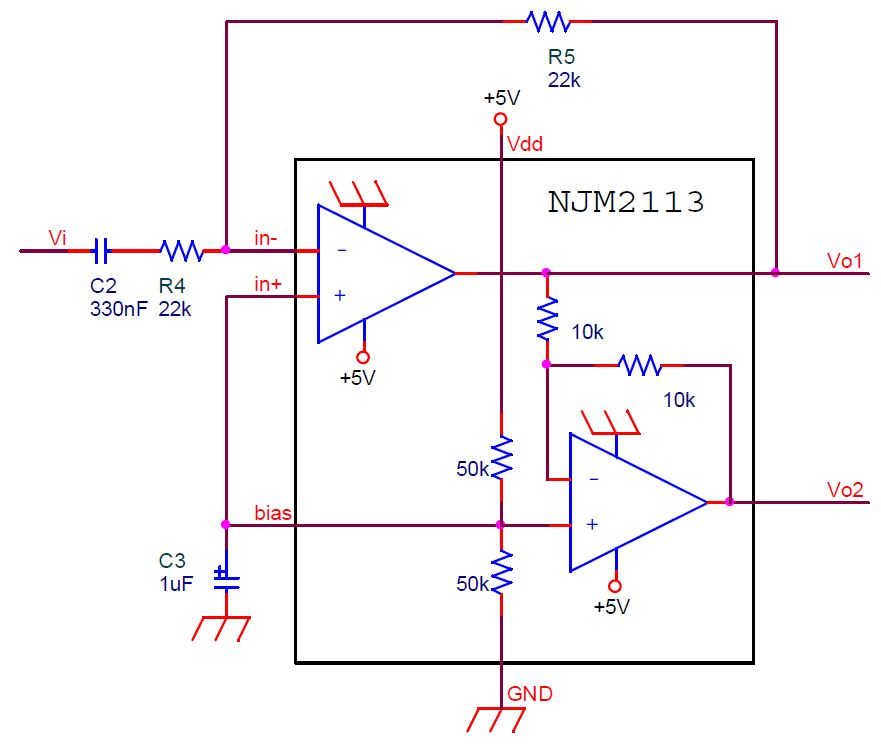
\includegraphics[scale=0.45]{NJM.JPG}
\label{LM4864}
\end{center}

Le circuit intégré (partie encadrée) contient : les 2 amplis-op, les résistances de rétroaction du 2\up{ème} ampli et un diviseur résistif pour créer la tension continue $E$ de $2,5V$.\\
Nous devons ajouter à l'extérieur : les résistances de rétroaction du 1\up{er} ampli, le condensateur du filtre passe-haut et un condensateur de grande valeur en parallèle sur la tension continue de $2,5V$ ($C_3$). Ce condensateur sert à stabiliser la tension continue (il forme un filtre passe-bas avec le diviseur résistif).


\subsection{Montage complet}
\Question{0}
{
%question
\textit{Maintenant que nous avons analysé tous les blocs du montage,
vérifiez que le gain total correspond bien à celui calculé à la sous-section \ref{analysepréliminaire}.}
}
{%assistant
$$G_{Total}=4.5\times 40=180$$, ce qui est même un peu plus que ce qui est nécessaire.
Pour éviter la saturation, il sera possible de régler le potentiomètre $R_{11}$ afin de légèrement diminuer le gain du troisième étage.
}

%\subsection{Illustration}
%Demandez à l'assistant de vous faire une démonstration de la fonction de filtrage.

%\clearpage
\newpage
\section*{ANNEXE A: Schéma de montage}
\label{montagetotal}
\begin{minipage}{.7\textwidth}
\begin{center}
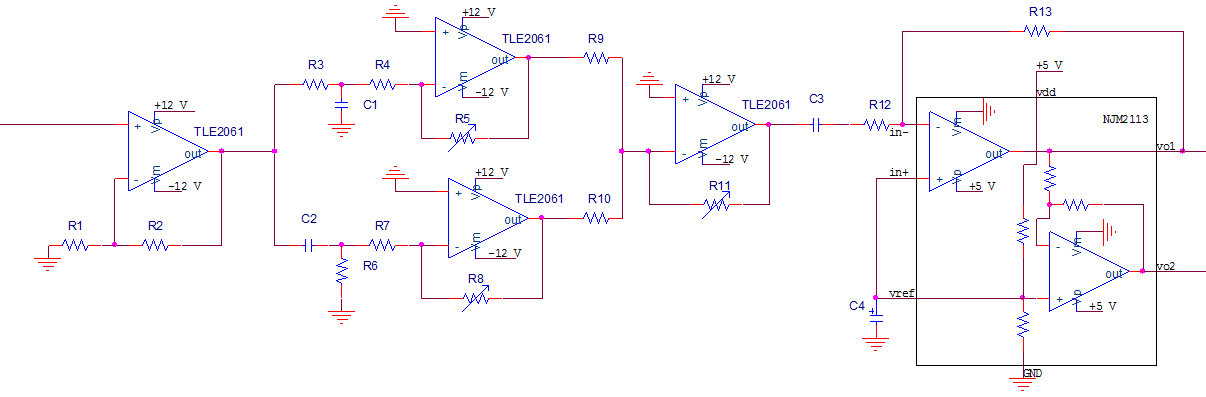
\includegraphics[width=23cm, angle=90]{circuittotal-non-annote.PNG}
\end{center}
\end{minipage}
\begin{minipage}{.25\textwidth}
\begin{center}
\rotatebox{90}{
\begin{tabular}{|c|c|c|c|c|c|}\hline
$R_1 = 1 k\Omega$ & $R_2 = 39 k\Omega$ & $R_3 = 2.7 k\Omega$ & $R_4 = 100 k\Omega$ & $R_5 = 100 k\Omega$ & $R_6 = 2.7 k\Omega$ \\ \hline
$R_7 = 100 k\Omega$ & $R_8 = 100 k\Omega$ & $R_9 = 22 k\Omega$ & $R_{10} = 22 k\Omega$ & $R_{11} = 100 k\Omega$ & $R_{12} = 22 k\Omega$ \\ \hline
$R_{13} = 22 k\Omega$ & $C_1 = 100 nF$ & $C_2 = 100 nF$ & $C_3 = 330 nF$ & $C_4 = 1 \mu F$ & \\ \hline
\end{tabular}
}
\end{center}
\end{minipage}


\section*{ANNEXE B: Datasheet TLE2061}
\vspace{-0.1cm}
\label{DatasheetCA3140}
\begin{center}
\includegraphics[scale=0.8, page=2]{tle2061.pdf}
\newpage
\includegraphics[scale=0.9, page=4]{tle2061.pdf}
\newpage
\includegraphics[scale=0.9, page=5]{tle2061.pdf}
\newpage
\includegraphics[scale=0.9, page=6]{tle2061.pdf}
\end{center}
\newpage


\endinput
